\documentclass[twoside]{book}

% Packages required by doxygen
\usepackage{fixltx2e}
\usepackage{calc}
\usepackage{doxygen}
\usepackage[export]{adjustbox} % also loads graphicx
\usepackage{graphicx}
\usepackage[utf8]{inputenc}
\usepackage{makeidx}
\usepackage{multicol}
\usepackage{multirow}
\PassOptionsToPackage{warn}{textcomp}
\usepackage{textcomp}
\usepackage[nointegrals]{wasysym}
\usepackage[table]{xcolor}

% Font selection
\usepackage[T1]{fontenc}
\usepackage[scaled=.90]{helvet}
\usepackage{courier}
\usepackage{amssymb}
\usepackage{sectsty}
\renewcommand{\familydefault}{\sfdefault}
\allsectionsfont{%
  \fontseries{bc}\selectfont%
  \color{darkgray}%
}
\renewcommand{\DoxyLabelFont}{%
  \fontseries{bc}\selectfont%
  \color{darkgray}%
}
\newcommand{\+}{\discretionary{\mbox{\scriptsize$\hookleftarrow$}}{}{}}

% Page & text layout
\usepackage{geometry}
\geometry{%
  a4paper,%
  top=2.5cm,%
  bottom=2.5cm,%
  left=2.5cm,%
  right=2.5cm%
}
\tolerance=750
\hfuzz=15pt
\hbadness=750
\setlength{\emergencystretch}{15pt}
\setlength{\parindent}{0cm}
\setlength{\parskip}{3ex plus 2ex minus 2ex}
\makeatletter
\renewcommand{\paragraph}{%
  \@startsection{paragraph}{4}{0ex}{-1.0ex}{1.0ex}{%
    \normalfont\normalsize\bfseries\SS@parafont%
  }%
}
\renewcommand{\subparagraph}{%
  \@startsection{subparagraph}{5}{0ex}{-1.0ex}{1.0ex}{%
    \normalfont\normalsize\bfseries\SS@subparafont%
  }%
}
\makeatother

% Headers & footers
\usepackage{fancyhdr}
\pagestyle{fancyplain}
\fancyhead[LE]{\fancyplain{}{\bfseries\thepage}}
\fancyhead[CE]{\fancyplain{}{}}
\fancyhead[RE]{\fancyplain{}{\bfseries\leftmark}}
\fancyhead[LO]{\fancyplain{}{\bfseries\rightmark}}
\fancyhead[CO]{\fancyplain{}{}}
\fancyhead[RO]{\fancyplain{}{\bfseries\thepage}}
\fancyfoot[LE]{\fancyplain{}{}}
\fancyfoot[CE]{\fancyplain{}{}}
\fancyfoot[RE]{\fancyplain{}{\bfseries\scriptsize Generated by Doxygen }}
\fancyfoot[LO]{\fancyplain{}{\bfseries\scriptsize Generated by Doxygen }}
\fancyfoot[CO]{\fancyplain{}{}}
\fancyfoot[RO]{\fancyplain{}{}}
\renewcommand{\footrulewidth}{0.4pt}
\renewcommand{\chaptermark}[1]{%
  \markboth{#1}{}%
}
\renewcommand{\sectionmark}[1]{%
  \markright{\thesection\ #1}%
}

% Indices & bibliography
\usepackage{natbib}
\usepackage[titles]{tocloft}
\setcounter{tocdepth}{3}
\setcounter{secnumdepth}{5}
\makeindex

% Custom commands
\newcommand{\clearemptydoublepage}{%
  \newpage{\pagestyle{empty}\cleardoublepage}%
}

\usepackage{caption}
\captionsetup{labelsep=space,justification=centering,font={bf},singlelinecheck=off,skip=4pt,position=top}

%===== C O N T E N T S =====

\begin{document}

% Titlepage & ToC
\pagenumbering{alph}
\begin{titlepage}
\vspace*{7cm}
\begin{center}%
{\Large Projet\+\_\+\+P5\+C006 }\\
\vspace*{1cm}
{\large Generated by Doxygen 1.8.14}\\
\end{center}
\end{titlepage}
\clearemptydoublepage
\pagenumbering{roman}
\tableofcontents
\clearemptydoublepage
\pagenumbering{arabic}

%--- Begin generated contents ---
\chapter{Namespace Index}
\section{Namespace List}
Here is a list of all namespaces with brief descriptions\+:\begin{DoxyCompactList}
\item\contentsline{section}{\textbf{ client} }{\pageref{namespaceclient}}{}
\item\contentsline{section}{\textbf{ graph\+IO} }{\pageref{namespacegraph_i_o}}{}
\item\contentsline{section}{\textbf{ hardy\+\_\+cross} }{\pageref{namespacehardy__cross}}{}
\item\contentsline{section}{\textbf{ kpi\+\_\+calculator} }{\pageref{namespacekpi__calculator}}{}
\item\contentsline{section}{\textbf{ router3} }{\pageref{namespacerouter3}}{}
\end{DoxyCompactList}

\chapter{Hierarchical Index}
\section{Class Hierarchy}
This inheritance list is sorted roughly, but not completely, alphabetically\+:\begin{DoxyCompactList}
\item \contentsline{section}{graph\+I\+O.\+display\+\_\+graph}{\pageref{classgraph_i_o_1_1display__graph}}{}
\item \contentsline{section}{graph\+I\+O.\+graph\+\_\+reader}{\pageref{classgraph_i_o_1_1graph__reader}}{}
\item \contentsline{section}{graph\+I\+O.\+graph\+\_\+writer}{\pageref{classgraph_i_o_1_1graph__writer}}{}
\item \contentsline{section}{kpi\+\_\+calculator.\+kpi\+\_\+calculator}{\pageref{classkpi__calculator_1_1kpi__calculator}}{}
\item object\begin{DoxyCompactList}
\item \contentsline{section}{hardy\+\_\+cross.\+Hardy\+Cross}{\pageref{classhardy__cross_1_1_hardy_cross}}{}
\item \contentsline{section}{router3.\+Router}{\pageref{classrouter3_1_1_router}}{}
\end{DoxyCompactList}
\end{DoxyCompactList}

\chapter{Class Index}
\section{Class List}
Here are the classes, structs, unions and interfaces with brief descriptions\+:\begin{DoxyCompactList}
\item\contentsline{section}{\textbf{ graph\+I\+O.\+display\+\_\+graph} }{\pageref{classgraph_i_o_1_1display__graph}}{}
\item\contentsline{section}{\textbf{ graph\+I\+O.\+graph\+\_\+reader} }{\pageref{classgraph_i_o_1_1graph__reader}}{}
\item\contentsline{section}{\textbf{ graph\+I\+O.\+graph\+\_\+writer} }{\pageref{classgraph_i_o_1_1graph__writer}}{}
\item\contentsline{section}{\textbf{ hardy\+\_\+cross.\+Hardy\+Cross} }{\pageref{classhardy__cross_1_1_hardy_cross}}{}
\item\contentsline{section}{\textbf{ kpi\+\_\+calculator.\+kpi\+\_\+calculator} }{\pageref{classkpi__calculator_1_1kpi__calculator}}{}
\item\contentsline{section}{\textbf{ router3.\+Router} }{\pageref{classrouter3_1_1_router}}{}
\end{DoxyCompactList}

\chapter{File Index}
\section{File List}
Here is a list of all files with brief descriptions\+:\begin{DoxyCompactList}
\item\contentsline{section}{source/\textbf{ client.\+py} }{\pageref{client_8py}}{}
\item\contentsline{section}{source/\textbf{ graph\+I\+O.\+py} }{\pageref{graph_i_o_8py}}{}
\item\contentsline{section}{source/\textbf{ hardy\+\_\+cross.\+py} }{\pageref{hardy__cross_8py}}{}
\item\contentsline{section}{source/\textbf{ kpi\+\_\+calculator.\+py} }{\pageref{kpi__calculator_8py}}{}
\item\contentsline{section}{source/\textbf{ router3.\+py} }{\pageref{router3_8py}}{}
\end{DoxyCompactList}

\chapter{Namespace Documentation}
\section{client Namespace Reference}
\label{namespaceclient}\index{client@{client}}
\subsection*{Functions}
\begin{DoxyCompactItemize}
\item 
def \textbf{ render\+\_\+vtk} (file\+\_\+name)
\item 
def \textbf{ vesuvio\+\_\+example} ()
\item 
def \textbf{ paesi\+\_\+example} ()
\item 
def \textbf{ casdetude} ()
\item 
def \textbf{ casdetude\+\_\+dinardo} ()
\item 
def \textbf{ adjacency\+\_\+matrix} ()
\item 
def \textbf{ automatic\+\_\+partitioning} ()
\end{DoxyCompactItemize}
\subsection*{Variables}
\begin{DoxyCompactItemize}
\item 
\textbf{ P\+R\+O\+J\+E\+C\+T\+\_\+\+P\+A\+TH} = os.\+path.\+dirname(os.\+path.\+abspath(\+\_\+\+\_\+file\+\_\+\+\_\+))
\item 
int \textbf{ last\+\_\+slash} = 0
\end{DoxyCompactItemize}


\subsection{Function Documentation}
\mbox{\label{namespaceclient_ab47128a10fdfd11ed5286a1d75370e4e}} 
\index{client@{client}!adjacency\+\_\+matrix@{adjacency\+\_\+matrix}}
\index{adjacency\+\_\+matrix@{adjacency\+\_\+matrix}!client@{client}}
\subsubsection{adjacency\+\_\+matrix()}
{\footnotesize\ttfamily def client.\+adjacency\+\_\+matrix (\begin{DoxyParamCaption}{ }\end{DoxyParamCaption})}

\begin{DoxyVerb}Imports a graph from an adjacency matrix and performs some spectra operations on it
\end{DoxyVerb}
 \mbox{\label{namespaceclient_aee49d67fb9021b0c97737423810ec697}} 
\index{client@{client}!automatic\+\_\+partitioning@{automatic\+\_\+partitioning}}
\index{automatic\+\_\+partitioning@{automatic\+\_\+partitioning}!client@{client}}
\subsubsection{automatic\+\_\+partitioning()}
{\footnotesize\ttfamily def client.\+automatic\+\_\+partitioning (\begin{DoxyParamCaption}{ }\end{DoxyParamCaption})}

\begin{DoxyVerb}Import a graph from an adjacency and runs the luvain comunity partitionig algorithm to find communites.
The result is show at screen
\end{DoxyVerb}
 \mbox{\label{namespaceclient_af8a75e716095fad89c5a359bbb43a2be}} 
\index{client@{client}!casdetude@{casdetude}}
\index{casdetude@{casdetude}!client@{client}}
\subsubsection{casdetude()}
{\footnotesize\ttfamily def client.\+casdetude (\begin{DoxyParamCaption}{ }\end{DoxyParamCaption})}

\begin{DoxyVerb}Imports the topograpy of the city of Monterusciello and automatically design the water supply network
\end{DoxyVerb}
 \mbox{\label{namespaceclient_aa98cb9a9cb0d62af6866771785480b53}} 
\index{client@{client}!casdetude\+\_\+dinardo@{casdetude\+\_\+dinardo}}
\index{casdetude\+\_\+dinardo@{casdetude\+\_\+dinardo}!client@{client}}
\subsubsection{casdetude\+\_\+dinardo()}
{\footnotesize\ttfamily def client.\+casdetude\+\_\+dinardo (\begin{DoxyParamCaption}{ }\end{DoxyParamCaption})}

\begin{DoxyVerb}Imports the topograpy of the city of Monterusciello and automatically design the water supply network
\end{DoxyVerb}
 \mbox{\label{namespaceclient_a9eec904ac0458c1bd157d5775c4e965b}} 
\index{client@{client}!paesi\+\_\+example@{paesi\+\_\+example}}
\index{paesi\+\_\+example@{paesi\+\_\+example}!client@{client}}
\subsubsection{paesi\+\_\+example()}
{\footnotesize\ttfamily def client.\+paesi\+\_\+example (\begin{DoxyParamCaption}{ }\end{DoxyParamCaption})}

\begin{DoxyVerb}Example of water distribution network partitioning.
The result is exported to a shapefile
\end{DoxyVerb}
 \mbox{\label{namespaceclient_a8c66f26b466cc16db7e35d978f747c1b}} 
\index{client@{client}!render\+\_\+vtk@{render\+\_\+vtk}}
\index{render\+\_\+vtk@{render\+\_\+vtk}!client@{client}}
\subsubsection{render\+\_\+vtk()}
{\footnotesize\ttfamily def client.\+render\+\_\+vtk (\begin{DoxyParamCaption}\item[{}]{file\+\_\+name }\end{DoxyParamCaption})}

\begin{DoxyVerb}Renders a vtk file
\end{DoxyVerb}
 \mbox{\label{namespaceclient_a46574221d0ff1ae8e8877b760085a01e}} 
\index{client@{client}!vesuvio\+\_\+example@{vesuvio\+\_\+example}}
\index{vesuvio\+\_\+example@{vesuvio\+\_\+example}!client@{client}}
\subsubsection{vesuvio\+\_\+example()}
{\footnotesize\ttfamily def client.\+vesuvio\+\_\+example (\begin{DoxyParamCaption}{ }\end{DoxyParamCaption})}

\begin{DoxyVerb}Example where the routing capabilities of the program are shown.
A topograpy of the vesuvio area is imported from a vtk file and the shortest path no it is calculated.
The result is than exported to vtk so that can be seen in paraview
\end{DoxyVerb}
 

\subsection{Variable Documentation}
\mbox{\label{namespaceclient_a4a7ede8654de42bed4384b998cad47b0}} 
\index{client@{client}!last\+\_\+slash@{last\+\_\+slash}}
\index{last\+\_\+slash@{last\+\_\+slash}!client@{client}}
\subsubsection{last\+\_\+slash}
{\footnotesize\ttfamily client.\+last\+\_\+slash = 0}

\mbox{\label{namespaceclient_ac4877b434d65a9c6830480ce21fd0b60}} 
\index{client@{client}!P\+R\+O\+J\+E\+C\+T\+\_\+\+P\+A\+TH@{P\+R\+O\+J\+E\+C\+T\+\_\+\+P\+A\+TH}}
\index{P\+R\+O\+J\+E\+C\+T\+\_\+\+P\+A\+TH@{P\+R\+O\+J\+E\+C\+T\+\_\+\+P\+A\+TH}!client@{client}}
\subsubsection{P\+R\+O\+J\+E\+C\+T\+\_\+\+P\+A\+TH}
{\footnotesize\ttfamily client.\+P\+R\+O\+J\+E\+C\+T\+\_\+\+P\+A\+TH = os.\+path.\+dirname(os.\+path.\+abspath(\+\_\+\+\_\+file\+\_\+\+\_\+))}


\section{graph\+IO Namespace Reference}
\label{namespacegraph_i_o}\index{graph\+IO@{graph\+IO}}
\subsection*{Classes}
\begin{DoxyCompactItemize}
\item 
class \textbf{ display\+\_\+graph}
\item 
class \textbf{ graph\+\_\+reader}
\item 
class \textbf{ graph\+\_\+writer}
\end{DoxyCompactItemize}

\section{hardy\+\_\+cross Namespace Reference}
\label{namespacehardy__cross}\index{hardy\+\_\+cross@{hardy\+\_\+cross}}
\subsection*{Classes}
\begin{DoxyCompactItemize}
\item 
class \textbf{ Hardy\+Cross}
\end{DoxyCompactItemize}
\subsection*{Functions}
\begin{DoxyCompactItemize}
\item 
def \textbf{ add\+\_\+string\+\_\+from\+\_\+list} (string\+\_\+list)
\item 
def \textbf{ flow\+\_\+correction\+\_\+dq} (df\+\_\+hf, df\+\_\+hf\+\_\+q)
\item 
def \textbf{ j\+\_\+loss\+\_\+10atm} (pipe\+\_\+diameter, flow\+\_\+rate)
\item 
def \textbf{ diameter\+\_\+from\+\_\+available} (theoretical\+\_\+diameter)
\item 
def \textbf{ diameter} (flow\+\_\+rate, velocity\+\_\+for\+\_\+diameter=0.\+8, show=0)
\item 
def \textbf{ velocity} (flow\+\_\+rate, pipe\+\_\+diameter)
\end{DoxyCompactItemize}


\subsection{Function Documentation}
\mbox{\label{namespacehardy__cross_af67df6b942deb06c74e8609dc5c32143}} 
\index{hardy\+\_\+cross@{hardy\+\_\+cross}!add\+\_\+string\+\_\+from\+\_\+list@{add\+\_\+string\+\_\+from\+\_\+list}}
\index{add\+\_\+string\+\_\+from\+\_\+list@{add\+\_\+string\+\_\+from\+\_\+list}!hardy\+\_\+cross@{hardy\+\_\+cross}}
\subsubsection{add\+\_\+string\+\_\+from\+\_\+list()}
{\footnotesize\ttfamily def hardy\+\_\+cross.\+add\+\_\+string\+\_\+from\+\_\+list (\begin{DoxyParamCaption}\item[{}]{string\+\_\+list }\end{DoxyParamCaption})}

\begin{DoxyVerb}:rtype : str
\end{DoxyVerb}
 \mbox{\label{namespacehardy__cross_a5b3a76084af3f0bb912856c7c3a297d0}} 
\index{hardy\+\_\+cross@{hardy\+\_\+cross}!diameter@{diameter}}
\index{diameter@{diameter}!hardy\+\_\+cross@{hardy\+\_\+cross}}
\subsubsection{diameter()}
{\footnotesize\ttfamily def hardy\+\_\+cross.\+diameter (\begin{DoxyParamCaption}\item[{}]{flow\+\_\+rate,  }\item[{}]{velocity\+\_\+for\+\_\+diameter = {\ttfamily 0.8},  }\item[{}]{show = {\ttfamily 0} }\end{DoxyParamCaption})}

\begin{DoxyVerb}Q: flow rate [l/s]
velocity_for_diameter: flow velocity m/s
D: diameter [mm]
\end{DoxyVerb}
 \mbox{\label{namespacehardy__cross_a554c5e38cee0615fabc782ad512e19e2}} 
\index{hardy\+\_\+cross@{hardy\+\_\+cross}!diameter\+\_\+from\+\_\+available@{diameter\+\_\+from\+\_\+available}}
\index{diameter\+\_\+from\+\_\+available@{diameter\+\_\+from\+\_\+available}!hardy\+\_\+cross@{hardy\+\_\+cross}}
\subsubsection{diameter\+\_\+from\+\_\+available()}
{\footnotesize\ttfamily def hardy\+\_\+cross.\+diameter\+\_\+from\+\_\+available (\begin{DoxyParamCaption}\item[{}]{theoretical\+\_\+diameter }\end{DoxyParamCaption})}

\mbox{\label{namespacehardy__cross_a62062bfea7848e6ebc3a6dd92f252e50}} 
\index{hardy\+\_\+cross@{hardy\+\_\+cross}!flow\+\_\+correction\+\_\+dq@{flow\+\_\+correction\+\_\+dq}}
\index{flow\+\_\+correction\+\_\+dq@{flow\+\_\+correction\+\_\+dq}!hardy\+\_\+cross@{hardy\+\_\+cross}}
\subsubsection{flow\+\_\+correction\+\_\+dq()}
{\footnotesize\ttfamily def hardy\+\_\+cross.\+flow\+\_\+correction\+\_\+dq (\begin{DoxyParamCaption}\item[{}]{df\+\_\+hf,  }\item[{}]{df\+\_\+hf\+\_\+q }\end{DoxyParamCaption})}

\begin{DoxyVerb}:type df_hf_q: float
:type df_hf: float
\end{DoxyVerb}
 \mbox{\label{namespacehardy__cross_aecaab5e3707cd3259ad7d21ff2fccbdd}} 
\index{hardy\+\_\+cross@{hardy\+\_\+cross}!j\+\_\+loss\+\_\+10atm@{j\+\_\+loss\+\_\+10atm}}
\index{j\+\_\+loss\+\_\+10atm@{j\+\_\+loss\+\_\+10atm}!hardy\+\_\+cross@{hardy\+\_\+cross}}
\subsubsection{j\+\_\+loss\+\_\+10atm()}
{\footnotesize\ttfamily def hardy\+\_\+cross.\+j\+\_\+loss\+\_\+10atm (\begin{DoxyParamCaption}\item[{}]{pipe\+\_\+diameter,  }\item[{}]{flow\+\_\+rate }\end{DoxyParamCaption})}

\begin{DoxyVerb}:param pipe_diameter: float
:param flow_rate: float
d: diameter [mm]
q: flow rate [l/s]
j: losses [m]
\end{DoxyVerb}
 \mbox{\label{namespacehardy__cross_a10c727ef7f7495f725c8d31d97d70ade}} 
\index{hardy\+\_\+cross@{hardy\+\_\+cross}!velocity@{velocity}}
\index{velocity@{velocity}!hardy\+\_\+cross@{hardy\+\_\+cross}}
\subsubsection{velocity()}
{\footnotesize\ttfamily def hardy\+\_\+cross.\+velocity (\begin{DoxyParamCaption}\item[{}]{flow\+\_\+rate,  }\item[{}]{pipe\+\_\+diameter }\end{DoxyParamCaption})}


\section{kpi\+\_\+calculator Namespace Reference}
\label{namespacekpi__calculator}\index{kpi\+\_\+calculator@{kpi\+\_\+calculator}}
\subsection*{Classes}
\begin{DoxyCompactItemize}
\item 
class \textbf{ kpi\+\_\+calculator}
\end{DoxyCompactItemize}

\section{router3 Namespace Reference}
\label{namespacerouter3}\index{router3@{router3}}
\subsection*{Classes}
\begin{DoxyCompactItemize}
\item 
class \textbf{ Router}
\end{DoxyCompactItemize}

\chapter{Class Documentation}
\section{graph\+I\+O.\+display\+\_\+graph Class Reference}
\label{classgraph_i_o_1_1display__graph}\index{graph\+I\+O.\+display\+\_\+graph@{graph\+I\+O.\+display\+\_\+graph}}
\subsection*{Public Member Functions}
\begin{DoxyCompactItemize}
\item 
def \textbf{ \+\_\+\+\_\+init\+\_\+\+\_\+} (self, \textbf{ graph})
\item 
def \textbf{ distance2D} (self, nodei, nodej)
\item 
def \textbf{ distance3D} (self, nodei, nodej)
\item 
def \textbf{ coord2D} (self, G)
\item 
def \textbf{ display\+\_\+mesh} (self)
\item 
def \textbf{ display\+\_\+path} (self, path)
\end{DoxyCompactItemize}
\subsection*{Public Attributes}
\begin{DoxyCompactItemize}
\item 
\textbf{ graph}
\end{DoxyCompactItemize}


\subsection{Detailed Description}
\begin{DoxyVerb}This class implements some usefull display function to plot the acqueduct a graph
\end{DoxyVerb}
 

\subsection{Constructor \& Destructor Documentation}
\mbox{\label{classgraph_i_o_1_1display__graph_a85738f48a8c587635575f205c85eb723}} 
\index{graph\+I\+O\+::display\+\_\+graph@{graph\+I\+O\+::display\+\_\+graph}!\+\_\+\+\_\+init\+\_\+\+\_\+@{\+\_\+\+\_\+init\+\_\+\+\_\+}}
\index{\+\_\+\+\_\+init\+\_\+\+\_\+@{\+\_\+\+\_\+init\+\_\+\+\_\+}!graph\+I\+O\+::display\+\_\+graph@{graph\+I\+O\+::display\+\_\+graph}}
\subsubsection{\+\_\+\+\_\+init\+\_\+\+\_\+()}
{\footnotesize\ttfamily def graph\+I\+O.\+display\+\_\+graph.\+\_\+\+\_\+init\+\_\+\+\_\+ (\begin{DoxyParamCaption}\item[{}]{self,  }\item[{}]{graph }\end{DoxyParamCaption})}



\subsection{Member Function Documentation}
\mbox{\label{classgraph_i_o_1_1display__graph_a332d64022b90bd947b73cb98570e6a43}} 
\index{graph\+I\+O\+::display\+\_\+graph@{graph\+I\+O\+::display\+\_\+graph}!coord2D@{coord2D}}
\index{coord2D@{coord2D}!graph\+I\+O\+::display\+\_\+graph@{graph\+I\+O\+::display\+\_\+graph}}
\subsubsection{coord2\+D()}
{\footnotesize\ttfamily def graph\+I\+O.\+display\+\_\+graph.\+coord2D (\begin{DoxyParamCaption}\item[{}]{self,  }\item[{}]{G }\end{DoxyParamCaption})}

\begin{DoxyVerb}Returns 2D coordinates of the nodes of self.graph
\end{DoxyVerb}
 \mbox{\label{classgraph_i_o_1_1display__graph_ab7c95142ba3a6606b44c122cbe6922b3}} 
\index{graph\+I\+O\+::display\+\_\+graph@{graph\+I\+O\+::display\+\_\+graph}!display\+\_\+mesh@{display\+\_\+mesh}}
\index{display\+\_\+mesh@{display\+\_\+mesh}!graph\+I\+O\+::display\+\_\+graph@{graph\+I\+O\+::display\+\_\+graph}}
\subsubsection{display\+\_\+mesh()}
{\footnotesize\ttfamily def graph\+I\+O.\+display\+\_\+graph.\+display\+\_\+mesh (\begin{DoxyParamCaption}\item[{}]{self }\end{DoxyParamCaption})}

\mbox{\label{classgraph_i_o_1_1display__graph_a16e2edb2ff0a29891861356ee70138b0}} 
\index{graph\+I\+O\+::display\+\_\+graph@{graph\+I\+O\+::display\+\_\+graph}!display\+\_\+path@{display\+\_\+path}}
\index{display\+\_\+path@{display\+\_\+path}!graph\+I\+O\+::display\+\_\+graph@{graph\+I\+O\+::display\+\_\+graph}}
\subsubsection{display\+\_\+path()}
{\footnotesize\ttfamily def graph\+I\+O.\+display\+\_\+graph.\+display\+\_\+path (\begin{DoxyParamCaption}\item[{}]{self,  }\item[{}]{path }\end{DoxyParamCaption})}

\begin{DoxyVerb}Display the mesh with a path marked on it
\end{DoxyVerb}
 \mbox{\label{classgraph_i_o_1_1display__graph_a63bdf36d35f077eb73abdb2bf0a7140e}} 
\index{graph\+I\+O\+::display\+\_\+graph@{graph\+I\+O\+::display\+\_\+graph}!distance2D@{distance2D}}
\index{distance2D@{distance2D}!graph\+I\+O\+::display\+\_\+graph@{graph\+I\+O\+::display\+\_\+graph}}
\subsubsection{distance2\+D()}
{\footnotesize\ttfamily def graph\+I\+O.\+display\+\_\+graph.\+distance2D (\begin{DoxyParamCaption}\item[{}]{self,  }\item[{}]{nodei,  }\item[{}]{nodej }\end{DoxyParamCaption})}

\begin{DoxyVerb}Computes the cartesian norme in 2D
\end{DoxyVerb}
 \mbox{\label{classgraph_i_o_1_1display__graph_a05bf3472530788eec304a3326815025c}} 
\index{graph\+I\+O\+::display\+\_\+graph@{graph\+I\+O\+::display\+\_\+graph}!distance3D@{distance3D}}
\index{distance3D@{distance3D}!graph\+I\+O\+::display\+\_\+graph@{graph\+I\+O\+::display\+\_\+graph}}
\subsubsection{distance3\+D()}
{\footnotesize\ttfamily def graph\+I\+O.\+display\+\_\+graph.\+distance3D (\begin{DoxyParamCaption}\item[{}]{self,  }\item[{}]{nodei,  }\item[{}]{nodej }\end{DoxyParamCaption})}

\begin{DoxyVerb}Computes the cartesian norme in 3D
\end{DoxyVerb}
 

\subsection{Member Data Documentation}
\mbox{\label{classgraph_i_o_1_1display__graph_a3140297ed4f443ab86216214b9f8d1f6}} 
\index{graph\+I\+O\+::display\+\_\+graph@{graph\+I\+O\+::display\+\_\+graph}!graph@{graph}}
\index{graph@{graph}!graph\+I\+O\+::display\+\_\+graph@{graph\+I\+O\+::display\+\_\+graph}}
\subsubsection{graph}
{\footnotesize\ttfamily graph\+I\+O.\+display\+\_\+graph.\+graph}



The documentation for this class was generated from the following file\+:\begin{DoxyCompactItemize}
\item 
source/\textbf{ graph\+I\+O.\+py}\end{DoxyCompactItemize}

\section{graph\+I\+O.\+graph\+\_\+reader Class Reference}
\label{classgraph_i_o_1_1graph__reader}\index{graph\+I\+O.\+graph\+\_\+reader@{graph\+I\+O.\+graph\+\_\+reader}}
\subsection*{Public Member Functions}
\begin{DoxyCompactItemize}
\item 
def \textbf{ \+\_\+\+\_\+init\+\_\+\+\_\+} (self, \textbf{ graph})
\item 
def \textbf{ avg} (self, node\+\_\+list)
\item 
def \textbf{ read\+\_\+shp\+\_\+bilding} (self, file\+\_\+name)
\item 
def \textbf{ row\+\_\+chuncker} (self, array, p\+\_\+array)
\item 
def \textbf{ read\+\_\+shp} (self, file\+\_\+name, point\+\_\+file=None)
\item 
def \textbf{ read\+\_\+adjacency} (self, filename)
\item 
def \textbf{ read\+\_\+epanet} (self, filename)
\end{DoxyCompactItemize}
\subsection*{Public Attributes}
\begin{DoxyCompactItemize}
\item 
\textbf{ graph}
\end{DoxyCompactItemize}


\subsection{Detailed Description}
\begin{DoxyVerb}This class provides the functions for graph reading from a multitude of formats
\end{DoxyVerb}
 

\subsection{Constructor \& Destructor Documentation}
\mbox{\label{classgraph_i_o_1_1graph__reader_a53537ae6fab9301a9559043ccb80f07e}} 
\index{graph\+I\+O\+::graph\+\_\+reader@{graph\+I\+O\+::graph\+\_\+reader}!\+\_\+\+\_\+init\+\_\+\+\_\+@{\+\_\+\+\_\+init\+\_\+\+\_\+}}
\index{\+\_\+\+\_\+init\+\_\+\+\_\+@{\+\_\+\+\_\+init\+\_\+\+\_\+}!graph\+I\+O\+::graph\+\_\+reader@{graph\+I\+O\+::graph\+\_\+reader}}
\subsubsection{\+\_\+\+\_\+init\+\_\+\+\_\+()}
{\footnotesize\ttfamily def graph\+I\+O.\+graph\+\_\+reader.\+\_\+\+\_\+init\+\_\+\+\_\+ (\begin{DoxyParamCaption}\item[{}]{self,  }\item[{}]{graph }\end{DoxyParamCaption})}



\subsection{Member Function Documentation}
\mbox{\label{classgraph_i_o_1_1graph__reader_a8b981c3c0ae92d95bf93013adafbb949}} 
\index{graph\+I\+O\+::graph\+\_\+reader@{graph\+I\+O\+::graph\+\_\+reader}!avg@{avg}}
\index{avg@{avg}!graph\+I\+O\+::graph\+\_\+reader@{graph\+I\+O\+::graph\+\_\+reader}}
\subsubsection{avg()}
{\footnotesize\ttfamily def graph\+I\+O.\+graph\+\_\+reader.\+avg (\begin{DoxyParamCaption}\item[{}]{self,  }\item[{}]{node\+\_\+list }\end{DoxyParamCaption})}

\mbox{\label{classgraph_i_o_1_1graph__reader_a140fd99201863857edad3bc98e26edf0}} 
\index{graph\+I\+O\+::graph\+\_\+reader@{graph\+I\+O\+::graph\+\_\+reader}!read\+\_\+adjacency@{read\+\_\+adjacency}}
\index{read\+\_\+adjacency@{read\+\_\+adjacency}!graph\+I\+O\+::graph\+\_\+reader@{graph\+I\+O\+::graph\+\_\+reader}}
\subsubsection{read\+\_\+adjacency()}
{\footnotesize\ttfamily def graph\+I\+O.\+graph\+\_\+reader.\+read\+\_\+adjacency (\begin{DoxyParamCaption}\item[{}]{self,  }\item[{}]{filename }\end{DoxyParamCaption})}

\mbox{\label{classgraph_i_o_1_1graph__reader_aed93e74f041adc3d1ca15153eaff7ada}} 
\index{graph\+I\+O\+::graph\+\_\+reader@{graph\+I\+O\+::graph\+\_\+reader}!read\+\_\+epanet@{read\+\_\+epanet}}
\index{read\+\_\+epanet@{read\+\_\+epanet}!graph\+I\+O\+::graph\+\_\+reader@{graph\+I\+O\+::graph\+\_\+reader}}
\subsubsection{read\+\_\+epanet()}
{\footnotesize\ttfamily def graph\+I\+O.\+graph\+\_\+reader.\+read\+\_\+epanet (\begin{DoxyParamCaption}\item[{}]{self,  }\item[{}]{filename }\end{DoxyParamCaption})}

\mbox{\label{classgraph_i_o_1_1graph__reader_a944d0cebc05facbfe9d68c7aa69f9e84}} 
\index{graph\+I\+O\+::graph\+\_\+reader@{graph\+I\+O\+::graph\+\_\+reader}!read\+\_\+shp@{read\+\_\+shp}}
\index{read\+\_\+shp@{read\+\_\+shp}!graph\+I\+O\+::graph\+\_\+reader@{graph\+I\+O\+::graph\+\_\+reader}}
\subsubsection{read\+\_\+shp()}
{\footnotesize\ttfamily def graph\+I\+O.\+graph\+\_\+reader.\+read\+\_\+shp (\begin{DoxyParamCaption}\item[{}]{self,  }\item[{}]{file\+\_\+name,  }\item[{}]{point\+\_\+file = {\ttfamily None} }\end{DoxyParamCaption})}

\begin{DoxyVerb}Generates a networkx.DiGraph from shapefiles. Point geometries are
translated into nodes, lines into edges. Coordinate tuples are used as
keys. Attributes are preserved, line geometries are simplified into
start and end coordinates. Accepts a single shapefile or directory of
many shapefiles.

"The Esri Shapefile or simply a shapefile is a popular geospatial
vector data format for geographic information systems software."

Parameters
----------
path : file or string
   File, directory, or filename to read.

simplify:  bool
    If ``True``, simplify line geometries to start and end coordinates.
    If ``False``, and line feature geometry has multiple segments, the
    non-geometric attributes for that feature will be repeated for each
    edge comprising that feature.

Returns
-------
G : NetworkX graph

Examples
--------
>>> G=nx.read_shp('test.shp') # doctest: +SKIP

References
----------
.. [1] http://en.wikipedia.org/wiki/Shapefile
\end{DoxyVerb}
 \mbox{\label{classgraph_i_o_1_1graph__reader_a9a8e5a3d1e940f83fb725615ef87581a}} 
\index{graph\+I\+O\+::graph\+\_\+reader@{graph\+I\+O\+::graph\+\_\+reader}!read\+\_\+shp\+\_\+bilding@{read\+\_\+shp\+\_\+bilding}}
\index{read\+\_\+shp\+\_\+bilding@{read\+\_\+shp\+\_\+bilding}!graph\+I\+O\+::graph\+\_\+reader@{graph\+I\+O\+::graph\+\_\+reader}}
\subsubsection{read\+\_\+shp\+\_\+bilding()}
{\footnotesize\ttfamily def graph\+I\+O.\+graph\+\_\+reader.\+read\+\_\+shp\+\_\+bilding (\begin{DoxyParamCaption}\item[{}]{self,  }\item[{}]{file\+\_\+name }\end{DoxyParamCaption})}

\mbox{\label{classgraph_i_o_1_1graph__reader_a4e7e90f2750cf23f970622c2109fb815}} 
\index{graph\+I\+O\+::graph\+\_\+reader@{graph\+I\+O\+::graph\+\_\+reader}!row\+\_\+chuncker@{row\+\_\+chuncker}}
\index{row\+\_\+chuncker@{row\+\_\+chuncker}!graph\+I\+O\+::graph\+\_\+reader@{graph\+I\+O\+::graph\+\_\+reader}}
\subsubsection{row\+\_\+chuncker()}
{\footnotesize\ttfamily def graph\+I\+O.\+graph\+\_\+reader.\+row\+\_\+chuncker (\begin{DoxyParamCaption}\item[{}]{self,  }\item[{}]{array,  }\item[{}]{p\+\_\+array }\end{DoxyParamCaption})}



\subsection{Member Data Documentation}
\mbox{\label{classgraph_i_o_1_1graph__reader_a3d6099f589156a7c02fd7cf6430d9500}} 
\index{graph\+I\+O\+::graph\+\_\+reader@{graph\+I\+O\+::graph\+\_\+reader}!graph@{graph}}
\index{graph@{graph}!graph\+I\+O\+::graph\+\_\+reader@{graph\+I\+O\+::graph\+\_\+reader}}
\subsubsection{graph}
{\footnotesize\ttfamily graph\+I\+O.\+graph\+\_\+reader.\+graph}



The documentation for this class was generated from the following file\+:\begin{DoxyCompactItemize}
\item 
source/\textbf{ graph\+I\+O.\+py}\end{DoxyCompactItemize}

\section{graph\+I\+O.\+graph\+\_\+writer Class Reference}
\label{classgraph_i_o_1_1graph__writer}\index{graph\+I\+O.\+graph\+\_\+writer@{graph\+I\+O.\+graph\+\_\+writer}}


The documentation for this class was generated from the following file\+:\begin{DoxyCompactItemize}
\item 
source/\textbf{ graph\+I\+O.\+py}\end{DoxyCompactItemize}

\section{hardy\+\_\+cross.\+Hardy\+Cross Class Reference}
\label{classhardy__cross_1_1_hardy_cross}\index{hardy\+\_\+cross.\+Hardy\+Cross@{hardy\+\_\+cross.\+Hardy\+Cross}}
Inheritance diagram for hardy\+\_\+cross.\+Hardy\+Cross\+:\begin{figure}[H]
\begin{center}
\leavevmode
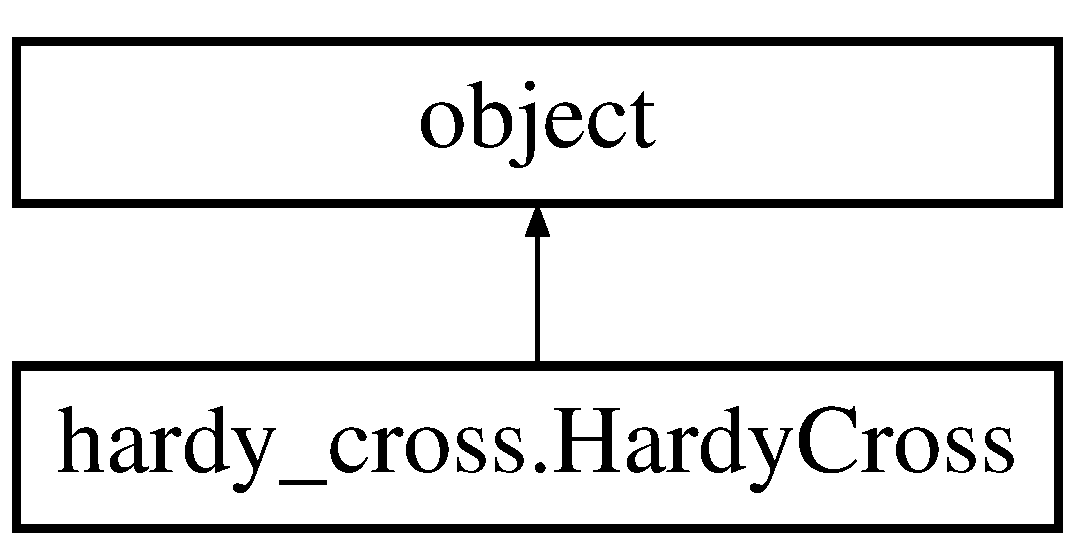
\includegraphics[height=2.000000cm]{classhardy__cross_1_1_hardy_cross}
\end{center}
\end{figure}
\subsection*{Public Member Functions}
\begin{DoxyCompactItemize}
\item 
def \textbf{ \+\_\+\+\_\+init\+\_\+\+\_\+} (self, \textbf{ loops})
\item 
def \textbf{ compute\+\_\+pipe\+\_\+diameter\+\_\+of\+\_\+each\+\_\+loop} (self)
\item 
def \textbf{ compute\+\_\+velocities\+\_\+of\+\_\+each\+\_\+loop} (self)
\item 
def \textbf{ sort\+\_\+edge\+\_\+names} (self)
\item 
def \textbf{ locate\+\_\+common\+\_\+loops} (self)
\item 
def \textbf{ run\+\_\+hc} (self)
\item 
def \textbf{ save\+\_\+flows\+\_\+to\+\_\+file} (self)
\end{DoxyCompactItemize}
\subsection*{Public Attributes}
\begin{DoxyCompactItemize}
\item 
\textbf{ runs}
\item 
\textbf{ threshold}
\item 
\textbf{ loops}
\item 
\textbf{ common\+\_\+loops}
\item 
\textbf{ delta\+\_\+\+Qs}
\item 
\textbf{ velocities}
\item 
\textbf{ new\+\_\+D}
\item 
\textbf{ smallest\+\_\+flow\+\_\+rate}
\item 
\textbf{ max\+\_\+velocity}
\item 
\textbf{ min\+\_\+velocity}
\end{DoxyCompactItemize}


\subsection{Constructor \& Destructor Documentation}
\mbox{\label{classhardy__cross_1_1_hardy_cross_a888eccf571149a93fdd02168eef2cc91}} 
\index{hardy\+\_\+cross\+::\+Hardy\+Cross@{hardy\+\_\+cross\+::\+Hardy\+Cross}!\+\_\+\+\_\+init\+\_\+\+\_\+@{\+\_\+\+\_\+init\+\_\+\+\_\+}}
\index{\+\_\+\+\_\+init\+\_\+\+\_\+@{\+\_\+\+\_\+init\+\_\+\+\_\+}!hardy\+\_\+cross\+::\+Hardy\+Cross@{hardy\+\_\+cross\+::\+Hardy\+Cross}}
\subsubsection{\+\_\+\+\_\+init\+\_\+\+\_\+()}
{\footnotesize\ttfamily def hardy\+\_\+cross.\+Hardy\+Cross.\+\_\+\+\_\+init\+\_\+\+\_\+ (\begin{DoxyParamCaption}\item[{}]{self,  }\item[{}]{loops }\end{DoxyParamCaption})}



\subsection{Member Function Documentation}
\mbox{\label{classhardy__cross_1_1_hardy_cross_a403abb80396de20a215d239d936efa04}} 
\index{hardy\+\_\+cross\+::\+Hardy\+Cross@{hardy\+\_\+cross\+::\+Hardy\+Cross}!compute\+\_\+pipe\+\_\+diameter\+\_\+of\+\_\+each\+\_\+loop@{compute\+\_\+pipe\+\_\+diameter\+\_\+of\+\_\+each\+\_\+loop}}
\index{compute\+\_\+pipe\+\_\+diameter\+\_\+of\+\_\+each\+\_\+loop@{compute\+\_\+pipe\+\_\+diameter\+\_\+of\+\_\+each\+\_\+loop}!hardy\+\_\+cross\+::\+Hardy\+Cross@{hardy\+\_\+cross\+::\+Hardy\+Cross}}
\subsubsection{compute\+\_\+pipe\+\_\+diameter\+\_\+of\+\_\+each\+\_\+loop()}
{\footnotesize\ttfamily def hardy\+\_\+cross.\+Hardy\+Cross.\+compute\+\_\+pipe\+\_\+diameter\+\_\+of\+\_\+each\+\_\+loop (\begin{DoxyParamCaption}\item[{}]{self }\end{DoxyParamCaption})}

\mbox{\label{classhardy__cross_1_1_hardy_cross_aaeaf69ae63839b27f154b3492a80c743}} 
\index{hardy\+\_\+cross\+::\+Hardy\+Cross@{hardy\+\_\+cross\+::\+Hardy\+Cross}!compute\+\_\+velocities\+\_\+of\+\_\+each\+\_\+loop@{compute\+\_\+velocities\+\_\+of\+\_\+each\+\_\+loop}}
\index{compute\+\_\+velocities\+\_\+of\+\_\+each\+\_\+loop@{compute\+\_\+velocities\+\_\+of\+\_\+each\+\_\+loop}!hardy\+\_\+cross\+::\+Hardy\+Cross@{hardy\+\_\+cross\+::\+Hardy\+Cross}}
\subsubsection{compute\+\_\+velocities\+\_\+of\+\_\+each\+\_\+loop()}
{\footnotesize\ttfamily def hardy\+\_\+cross.\+Hardy\+Cross.\+compute\+\_\+velocities\+\_\+of\+\_\+each\+\_\+loop (\begin{DoxyParamCaption}\item[{}]{self }\end{DoxyParamCaption})}

\mbox{\label{classhardy__cross_1_1_hardy_cross_a7ca4aa87024f6d117e0b9693bd05a058}} 
\index{hardy\+\_\+cross\+::\+Hardy\+Cross@{hardy\+\_\+cross\+::\+Hardy\+Cross}!locate\+\_\+common\+\_\+loops@{locate\+\_\+common\+\_\+loops}}
\index{locate\+\_\+common\+\_\+loops@{locate\+\_\+common\+\_\+loops}!hardy\+\_\+cross\+::\+Hardy\+Cross@{hardy\+\_\+cross\+::\+Hardy\+Cross}}
\subsubsection{locate\+\_\+common\+\_\+loops()}
{\footnotesize\ttfamily def hardy\+\_\+cross.\+Hardy\+Cross.\+locate\+\_\+common\+\_\+loops (\begin{DoxyParamCaption}\item[{}]{self }\end{DoxyParamCaption})}

\begin{DoxyVerb}this method locates the common edges and for each loop it creates a sparce matrix/array where the common edge/s
is symbolized by the number 1. each matrix later will be multiplied (dot) by the delta_Qs.
:return: None
\end{DoxyVerb}
 \mbox{\label{classhardy__cross_1_1_hardy_cross_a508fc873ca07138a7f6caec2dc6f5e83}} 
\index{hardy\+\_\+cross\+::\+Hardy\+Cross@{hardy\+\_\+cross\+::\+Hardy\+Cross}!run\+\_\+hc@{run\+\_\+hc}}
\index{run\+\_\+hc@{run\+\_\+hc}!hardy\+\_\+cross\+::\+Hardy\+Cross@{hardy\+\_\+cross\+::\+Hardy\+Cross}}
\subsubsection{run\+\_\+hc()}
{\footnotesize\ttfamily def hardy\+\_\+cross.\+Hardy\+Cross.\+run\+\_\+hc (\begin{DoxyParamCaption}\item[{}]{self }\end{DoxyParamCaption})}

\mbox{\label{classhardy__cross_1_1_hardy_cross_ac7bb55de1f73da2011b60e39ba79b6a1}} 
\index{hardy\+\_\+cross\+::\+Hardy\+Cross@{hardy\+\_\+cross\+::\+Hardy\+Cross}!save\+\_\+flows\+\_\+to\+\_\+file@{save\+\_\+flows\+\_\+to\+\_\+file}}
\index{save\+\_\+flows\+\_\+to\+\_\+file@{save\+\_\+flows\+\_\+to\+\_\+file}!hardy\+\_\+cross\+::\+Hardy\+Cross@{hardy\+\_\+cross\+::\+Hardy\+Cross}}
\subsubsection{save\+\_\+flows\+\_\+to\+\_\+file()}
{\footnotesize\ttfamily def hardy\+\_\+cross.\+Hardy\+Cross.\+save\+\_\+flows\+\_\+to\+\_\+file (\begin{DoxyParamCaption}\item[{}]{self }\end{DoxyParamCaption})}

\mbox{\label{classhardy__cross_1_1_hardy_cross_a2758df038b7f5484310be5667071bae6}} 
\index{hardy\+\_\+cross\+::\+Hardy\+Cross@{hardy\+\_\+cross\+::\+Hardy\+Cross}!sort\+\_\+edge\+\_\+names@{sort\+\_\+edge\+\_\+names}}
\index{sort\+\_\+edge\+\_\+names@{sort\+\_\+edge\+\_\+names}!hardy\+\_\+cross\+::\+Hardy\+Cross@{hardy\+\_\+cross\+::\+Hardy\+Cross}}
\subsubsection{sort\+\_\+edge\+\_\+names()}
{\footnotesize\ttfamily def hardy\+\_\+cross.\+Hardy\+Cross.\+sort\+\_\+edge\+\_\+names (\begin{DoxyParamCaption}\item[{}]{self }\end{DoxyParamCaption})}



\subsection{Member Data Documentation}
\mbox{\label{classhardy__cross_1_1_hardy_cross_a7d71de8073fad4c23e1395b146ac2bfc}} 
\index{hardy\+\_\+cross\+::\+Hardy\+Cross@{hardy\+\_\+cross\+::\+Hardy\+Cross}!common\+\_\+loops@{common\+\_\+loops}}
\index{common\+\_\+loops@{common\+\_\+loops}!hardy\+\_\+cross\+::\+Hardy\+Cross@{hardy\+\_\+cross\+::\+Hardy\+Cross}}
\subsubsection{common\+\_\+loops}
{\footnotesize\ttfamily hardy\+\_\+cross.\+Hardy\+Cross.\+common\+\_\+loops}

\mbox{\label{classhardy__cross_1_1_hardy_cross_aeed85466161aeb75d564538abc2a2a2c}} 
\index{hardy\+\_\+cross\+::\+Hardy\+Cross@{hardy\+\_\+cross\+::\+Hardy\+Cross}!delta\+\_\+\+Qs@{delta\+\_\+\+Qs}}
\index{delta\+\_\+\+Qs@{delta\+\_\+\+Qs}!hardy\+\_\+cross\+::\+Hardy\+Cross@{hardy\+\_\+cross\+::\+Hardy\+Cross}}
\subsubsection{delta\+\_\+\+Qs}
{\footnotesize\ttfamily hardy\+\_\+cross.\+Hardy\+Cross.\+delta\+\_\+\+Qs}

\mbox{\label{classhardy__cross_1_1_hardy_cross_ab99990c6b58750559ad55d66d7f1ddcb}} 
\index{hardy\+\_\+cross\+::\+Hardy\+Cross@{hardy\+\_\+cross\+::\+Hardy\+Cross}!loops@{loops}}
\index{loops@{loops}!hardy\+\_\+cross\+::\+Hardy\+Cross@{hardy\+\_\+cross\+::\+Hardy\+Cross}}
\subsubsection{loops}
{\footnotesize\ttfamily hardy\+\_\+cross.\+Hardy\+Cross.\+loops}

\mbox{\label{classhardy__cross_1_1_hardy_cross_ac59be31a2d76269fe0734257dc53525e}} 
\index{hardy\+\_\+cross\+::\+Hardy\+Cross@{hardy\+\_\+cross\+::\+Hardy\+Cross}!max\+\_\+velocity@{max\+\_\+velocity}}
\index{max\+\_\+velocity@{max\+\_\+velocity}!hardy\+\_\+cross\+::\+Hardy\+Cross@{hardy\+\_\+cross\+::\+Hardy\+Cross}}
\subsubsection{max\+\_\+velocity}
{\footnotesize\ttfamily hardy\+\_\+cross.\+Hardy\+Cross.\+max\+\_\+velocity}

\mbox{\label{classhardy__cross_1_1_hardy_cross_a3debd53378e986f10b8614608d11884c}} 
\index{hardy\+\_\+cross\+::\+Hardy\+Cross@{hardy\+\_\+cross\+::\+Hardy\+Cross}!min\+\_\+velocity@{min\+\_\+velocity}}
\index{min\+\_\+velocity@{min\+\_\+velocity}!hardy\+\_\+cross\+::\+Hardy\+Cross@{hardy\+\_\+cross\+::\+Hardy\+Cross}}
\subsubsection{min\+\_\+velocity}
{\footnotesize\ttfamily hardy\+\_\+cross.\+Hardy\+Cross.\+min\+\_\+velocity}

\mbox{\label{classhardy__cross_1_1_hardy_cross_af15396e4d0cde2e779eed7c2f46b20ea}} 
\index{hardy\+\_\+cross\+::\+Hardy\+Cross@{hardy\+\_\+cross\+::\+Hardy\+Cross}!new\+\_\+D@{new\+\_\+D}}
\index{new\+\_\+D@{new\+\_\+D}!hardy\+\_\+cross\+::\+Hardy\+Cross@{hardy\+\_\+cross\+::\+Hardy\+Cross}}
\subsubsection{new\+\_\+D}
{\footnotesize\ttfamily hardy\+\_\+cross.\+Hardy\+Cross.\+new\+\_\+D}

\mbox{\label{classhardy__cross_1_1_hardy_cross_adafc07a3a8284be3fe499df624b370e4}} 
\index{hardy\+\_\+cross\+::\+Hardy\+Cross@{hardy\+\_\+cross\+::\+Hardy\+Cross}!runs@{runs}}
\index{runs@{runs}!hardy\+\_\+cross\+::\+Hardy\+Cross@{hardy\+\_\+cross\+::\+Hardy\+Cross}}
\subsubsection{runs}
{\footnotesize\ttfamily hardy\+\_\+cross.\+Hardy\+Cross.\+runs}

\mbox{\label{classhardy__cross_1_1_hardy_cross_a7da2766104b1c265ca1a6a556ca4cdbc}} 
\index{hardy\+\_\+cross\+::\+Hardy\+Cross@{hardy\+\_\+cross\+::\+Hardy\+Cross}!smallest\+\_\+flow\+\_\+rate@{smallest\+\_\+flow\+\_\+rate}}
\index{smallest\+\_\+flow\+\_\+rate@{smallest\+\_\+flow\+\_\+rate}!hardy\+\_\+cross\+::\+Hardy\+Cross@{hardy\+\_\+cross\+::\+Hardy\+Cross}}
\subsubsection{smallest\+\_\+flow\+\_\+rate}
{\footnotesize\ttfamily hardy\+\_\+cross.\+Hardy\+Cross.\+smallest\+\_\+flow\+\_\+rate}

\mbox{\label{classhardy__cross_1_1_hardy_cross_ab508a75b06e13bd36848e65f87be3acd}} 
\index{hardy\+\_\+cross\+::\+Hardy\+Cross@{hardy\+\_\+cross\+::\+Hardy\+Cross}!threshold@{threshold}}
\index{threshold@{threshold}!hardy\+\_\+cross\+::\+Hardy\+Cross@{hardy\+\_\+cross\+::\+Hardy\+Cross}}
\subsubsection{threshold}
{\footnotesize\ttfamily hardy\+\_\+cross.\+Hardy\+Cross.\+threshold}

\mbox{\label{classhardy__cross_1_1_hardy_cross_a925d9a4ce1572b2ec3bbccc8646517e9}} 
\index{hardy\+\_\+cross\+::\+Hardy\+Cross@{hardy\+\_\+cross\+::\+Hardy\+Cross}!velocities@{velocities}}
\index{velocities@{velocities}!hardy\+\_\+cross\+::\+Hardy\+Cross@{hardy\+\_\+cross\+::\+Hardy\+Cross}}
\subsubsection{velocities}
{\footnotesize\ttfamily hardy\+\_\+cross.\+Hardy\+Cross.\+velocities}



The documentation for this class was generated from the following file\+:\begin{DoxyCompactItemize}
\item 
source/\textbf{ hardy\+\_\+cross.\+py}\end{DoxyCompactItemize}

\section{kpi\+\_\+calculator.\+kpi\+\_\+calculator Class Reference}
\label{classkpi__calculator_1_1kpi__calculator}\index{kpi\+\_\+calculator.\+kpi\+\_\+calculator@{kpi\+\_\+calculator.\+kpi\+\_\+calculator}}
\subsection*{Public Member Functions}
\begin{DoxyCompactItemize}
\item 
def \textbf{ \+\_\+\+\_\+init\+\_\+\+\_\+} (self, \textbf{ wdn})
\item 
def \textbf{ print\+\_\+kpi} (self)
\end{DoxyCompactItemize}
\subsection*{Public Attributes}
\begin{DoxyCompactItemize}
\item 
\textbf{ available\+\_\+power}
\item 
\textbf{ dissipated\+\_\+power}
\item 
\textbf{ nodes\+\_\+power}
\item 
\textbf{ M\+IN}
\item 
\textbf{ M\+AX}
\end{DoxyCompactItemize}
\subsection*{Static Public Attributes}
\begin{DoxyCompactItemize}
\item 
\textbf{ wdn} = nx.\+Graph()
\item 
int \textbf{ available\+\_\+power} = 0
\item 
int \textbf{ dissipated\+\_\+power} = 0
\item 
list \textbf{ M\+IN} = [$\,$]
\item 
list \textbf{ M\+AX} = [$\,$]
\item 
list \textbf{ M\+E\+AN} = [$\,$]
\item 
list \textbf{ S\+QM} = [$\,$]
\end{DoxyCompactItemize}


\subsection{Detailed Description}
\begin{DoxyVerb}This class computes performance indicators for a solved water distribuion network.
Varius types of indicators are available:
- Energy indicators of the network
    - available_power
    - dissipated_power
- Statistical indicators of nodes head per cluster
    - min
    - max
    - mean
    - mean square error
\end{DoxyVerb}
 

\subsection{Constructor \& Destructor Documentation}
\mbox{\label{classkpi__calculator_1_1kpi__calculator_a66803ce7419ea76b9c26f7e280acec6f}} 
\index{kpi\+\_\+calculator\+::kpi\+\_\+calculator@{kpi\+\_\+calculator\+::kpi\+\_\+calculator}!\+\_\+\+\_\+init\+\_\+\+\_\+@{\+\_\+\+\_\+init\+\_\+\+\_\+}}
\index{\+\_\+\+\_\+init\+\_\+\+\_\+@{\+\_\+\+\_\+init\+\_\+\+\_\+}!kpi\+\_\+calculator\+::kpi\+\_\+calculator@{kpi\+\_\+calculator\+::kpi\+\_\+calculator}}
\subsubsection{\+\_\+\+\_\+init\+\_\+\+\_\+()}
{\footnotesize\ttfamily def kpi\+\_\+calculator.\+kpi\+\_\+calculator.\+\_\+\+\_\+init\+\_\+\+\_\+ (\begin{DoxyParamCaption}\item[{}]{self,  }\item[{}]{wdn }\end{DoxyParamCaption})}



\subsection{Member Function Documentation}
\mbox{\label{classkpi__calculator_1_1kpi__calculator_a1662784590b32c7c1866809e7fca6b61}} 
\index{kpi\+\_\+calculator\+::kpi\+\_\+calculator@{kpi\+\_\+calculator\+::kpi\+\_\+calculator}!print\+\_\+kpi@{print\+\_\+kpi}}
\index{print\+\_\+kpi@{print\+\_\+kpi}!kpi\+\_\+calculator\+::kpi\+\_\+calculator@{kpi\+\_\+calculator\+::kpi\+\_\+calculator}}
\subsubsection{print\+\_\+kpi()}
{\footnotesize\ttfamily def kpi\+\_\+calculator.\+kpi\+\_\+calculator.\+print\+\_\+kpi (\begin{DoxyParamCaption}\item[{}]{self }\end{DoxyParamCaption})}



\subsection{Member Data Documentation}
\mbox{\label{classkpi__calculator_1_1kpi__calculator_ad2051fd25f5819976a92b7ba7c32ebae}} 
\index{kpi\+\_\+calculator\+::kpi\+\_\+calculator@{kpi\+\_\+calculator\+::kpi\+\_\+calculator}!available\+\_\+power@{available\+\_\+power}}
\index{available\+\_\+power@{available\+\_\+power}!kpi\+\_\+calculator\+::kpi\+\_\+calculator@{kpi\+\_\+calculator\+::kpi\+\_\+calculator}}
\subsubsection{available\+\_\+power\hspace{0.1cm}{\footnotesize\ttfamily [1/2]}}
{\footnotesize\ttfamily int kpi\+\_\+calculator.\+kpi\+\_\+calculator.\+available\+\_\+power = 0\hspace{0.3cm}{\ttfamily [static]}}

\mbox{\label{classkpi__calculator_1_1kpi__calculator_a579ab05f33e7e638d4f8bafec0b8d81f}} 
\index{kpi\+\_\+calculator\+::kpi\+\_\+calculator@{kpi\+\_\+calculator\+::kpi\+\_\+calculator}!available\+\_\+power@{available\+\_\+power}}
\index{available\+\_\+power@{available\+\_\+power}!kpi\+\_\+calculator\+::kpi\+\_\+calculator@{kpi\+\_\+calculator\+::kpi\+\_\+calculator}}
\subsubsection{available\+\_\+power\hspace{0.1cm}{\footnotesize\ttfamily [2/2]}}
{\footnotesize\ttfamily kpi\+\_\+calculator.\+kpi\+\_\+calculator.\+available\+\_\+power}

\mbox{\label{classkpi__calculator_1_1kpi__calculator_a10ea71c7cd818a982a3a5b02a6af1c01}} 
\index{kpi\+\_\+calculator\+::kpi\+\_\+calculator@{kpi\+\_\+calculator\+::kpi\+\_\+calculator}!dissipated\+\_\+power@{dissipated\+\_\+power}}
\index{dissipated\+\_\+power@{dissipated\+\_\+power}!kpi\+\_\+calculator\+::kpi\+\_\+calculator@{kpi\+\_\+calculator\+::kpi\+\_\+calculator}}
\subsubsection{dissipated\+\_\+power\hspace{0.1cm}{\footnotesize\ttfamily [1/2]}}
{\footnotesize\ttfamily int kpi\+\_\+calculator.\+kpi\+\_\+calculator.\+dissipated\+\_\+power = 0\hspace{0.3cm}{\ttfamily [static]}}

\mbox{\label{classkpi__calculator_1_1kpi__calculator_ab4753fbb14bb42b451a0563b0e3b874e}} 
\index{kpi\+\_\+calculator\+::kpi\+\_\+calculator@{kpi\+\_\+calculator\+::kpi\+\_\+calculator}!dissipated\+\_\+power@{dissipated\+\_\+power}}
\index{dissipated\+\_\+power@{dissipated\+\_\+power}!kpi\+\_\+calculator\+::kpi\+\_\+calculator@{kpi\+\_\+calculator\+::kpi\+\_\+calculator}}
\subsubsection{dissipated\+\_\+power\hspace{0.1cm}{\footnotesize\ttfamily [2/2]}}
{\footnotesize\ttfamily kpi\+\_\+calculator.\+kpi\+\_\+calculator.\+dissipated\+\_\+power}

\mbox{\label{classkpi__calculator_1_1kpi__calculator_afd709bd6a7d09ad358530b41bca549b8}} 
\index{kpi\+\_\+calculator\+::kpi\+\_\+calculator@{kpi\+\_\+calculator\+::kpi\+\_\+calculator}!M\+AX@{M\+AX}}
\index{M\+AX@{M\+AX}!kpi\+\_\+calculator\+::kpi\+\_\+calculator@{kpi\+\_\+calculator\+::kpi\+\_\+calculator}}
\subsubsection{M\+AX\hspace{0.1cm}{\footnotesize\ttfamily [1/2]}}
{\footnotesize\ttfamily list kpi\+\_\+calculator.\+kpi\+\_\+calculator.\+M\+AX = [$\,$]\hspace{0.3cm}{\ttfamily [static]}}

\mbox{\label{classkpi__calculator_1_1kpi__calculator_af0783131b393f842740b8da244f88c3d}} 
\index{kpi\+\_\+calculator\+::kpi\+\_\+calculator@{kpi\+\_\+calculator\+::kpi\+\_\+calculator}!M\+AX@{M\+AX}}
\index{M\+AX@{M\+AX}!kpi\+\_\+calculator\+::kpi\+\_\+calculator@{kpi\+\_\+calculator\+::kpi\+\_\+calculator}}
\subsubsection{M\+AX\hspace{0.1cm}{\footnotesize\ttfamily [2/2]}}
{\footnotesize\ttfamily kpi\+\_\+calculator.\+kpi\+\_\+calculator.\+M\+AX}

\mbox{\label{classkpi__calculator_1_1kpi__calculator_af4ab5c02b4eca487dbadea201b74d4ea}} 
\index{kpi\+\_\+calculator\+::kpi\+\_\+calculator@{kpi\+\_\+calculator\+::kpi\+\_\+calculator}!M\+E\+AN@{M\+E\+AN}}
\index{M\+E\+AN@{M\+E\+AN}!kpi\+\_\+calculator\+::kpi\+\_\+calculator@{kpi\+\_\+calculator\+::kpi\+\_\+calculator}}
\subsubsection{M\+E\+AN}
{\footnotesize\ttfamily list kpi\+\_\+calculator.\+kpi\+\_\+calculator.\+M\+E\+AN = [$\,$]\hspace{0.3cm}{\ttfamily [static]}}

\mbox{\label{classkpi__calculator_1_1kpi__calculator_a8ee4ae59c3f523247f7f028e67f571df}} 
\index{kpi\+\_\+calculator\+::kpi\+\_\+calculator@{kpi\+\_\+calculator\+::kpi\+\_\+calculator}!M\+IN@{M\+IN}}
\index{M\+IN@{M\+IN}!kpi\+\_\+calculator\+::kpi\+\_\+calculator@{kpi\+\_\+calculator\+::kpi\+\_\+calculator}}
\subsubsection{M\+IN\hspace{0.1cm}{\footnotesize\ttfamily [1/2]}}
{\footnotesize\ttfamily list kpi\+\_\+calculator.\+kpi\+\_\+calculator.\+M\+IN = [$\,$]\hspace{0.3cm}{\ttfamily [static]}}

\mbox{\label{classkpi__calculator_1_1kpi__calculator_a7c1c47bf6cf1db2fbde9a029d3ce7cf6}} 
\index{kpi\+\_\+calculator\+::kpi\+\_\+calculator@{kpi\+\_\+calculator\+::kpi\+\_\+calculator}!M\+IN@{M\+IN}}
\index{M\+IN@{M\+IN}!kpi\+\_\+calculator\+::kpi\+\_\+calculator@{kpi\+\_\+calculator\+::kpi\+\_\+calculator}}
\subsubsection{M\+IN\hspace{0.1cm}{\footnotesize\ttfamily [2/2]}}
{\footnotesize\ttfamily kpi\+\_\+calculator.\+kpi\+\_\+calculator.\+M\+IN}

\mbox{\label{classkpi__calculator_1_1kpi__calculator_af39d7b6b02347698aae38d60393a1ae5}} 
\index{kpi\+\_\+calculator\+::kpi\+\_\+calculator@{kpi\+\_\+calculator\+::kpi\+\_\+calculator}!nodes\+\_\+power@{nodes\+\_\+power}}
\index{nodes\+\_\+power@{nodes\+\_\+power}!kpi\+\_\+calculator\+::kpi\+\_\+calculator@{kpi\+\_\+calculator\+::kpi\+\_\+calculator}}
\subsubsection{nodes\+\_\+power}
{\footnotesize\ttfamily kpi\+\_\+calculator.\+kpi\+\_\+calculator.\+nodes\+\_\+power}

\mbox{\label{classkpi__calculator_1_1kpi__calculator_aa9ca35010865a3967de0326814ec61ec}} 
\index{kpi\+\_\+calculator\+::kpi\+\_\+calculator@{kpi\+\_\+calculator\+::kpi\+\_\+calculator}!S\+QM@{S\+QM}}
\index{S\+QM@{S\+QM}!kpi\+\_\+calculator\+::kpi\+\_\+calculator@{kpi\+\_\+calculator\+::kpi\+\_\+calculator}}
\subsubsection{S\+QM}
{\footnotesize\ttfamily list kpi\+\_\+calculator.\+kpi\+\_\+calculator.\+S\+QM = [$\,$]\hspace{0.3cm}{\ttfamily [static]}}

\mbox{\label{classkpi__calculator_1_1kpi__calculator_a5b302b617998b33d4caf1056144edcc6}} 
\index{kpi\+\_\+calculator\+::kpi\+\_\+calculator@{kpi\+\_\+calculator\+::kpi\+\_\+calculator}!wdn@{wdn}}
\index{wdn@{wdn}!kpi\+\_\+calculator\+::kpi\+\_\+calculator@{kpi\+\_\+calculator\+::kpi\+\_\+calculator}}
\subsubsection{wdn}
{\footnotesize\ttfamily kpi\+\_\+calculator.\+kpi\+\_\+calculator.\+wdn = nx.\+Graph()\hspace{0.3cm}{\ttfamily [static]}}



The documentation for this class was generated from the following file\+:\begin{DoxyCompactItemize}
\item 
source/\textbf{ kpi\+\_\+calculator.\+py}\end{DoxyCompactItemize}

\section{router3.\+Router Class Reference}
\label{classrouter3_1_1_router}\index{router3.\+Router@{router3.\+Router}}
Inheritance diagram for router3.\+Router\+:\begin{figure}[H]
\begin{center}
\leavevmode
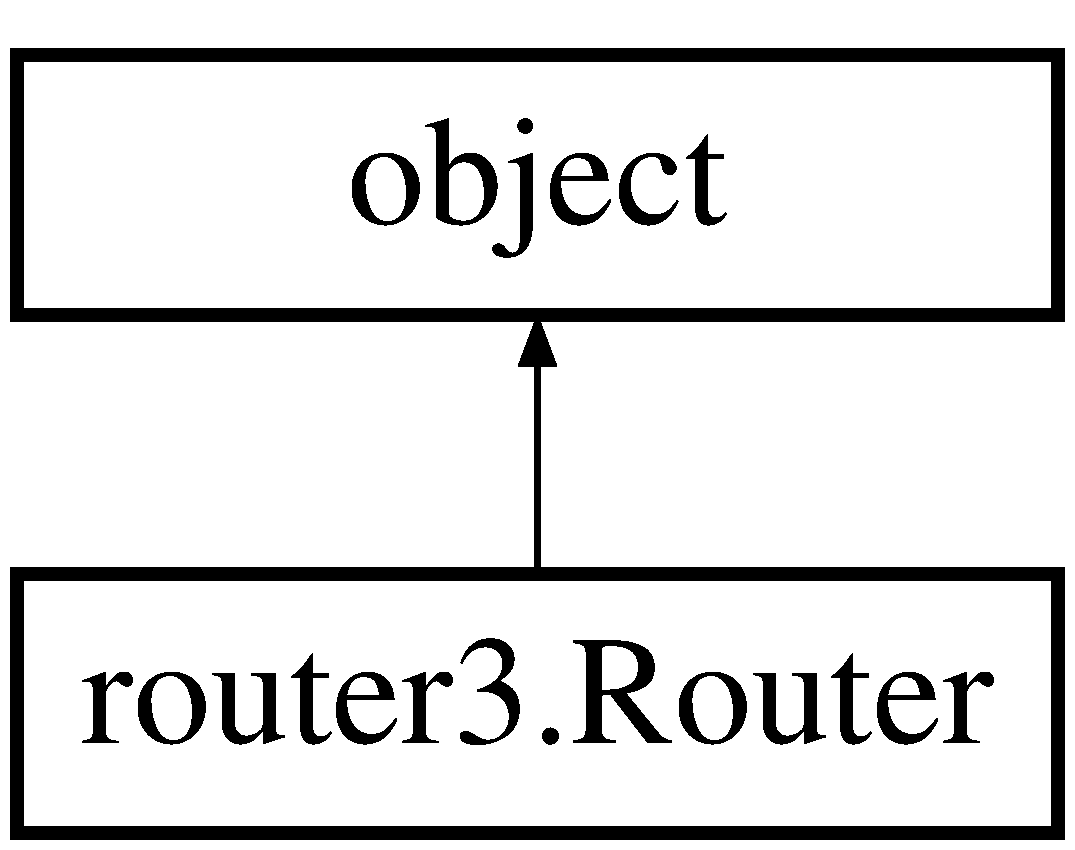
\includegraphics[height=2.000000cm]{classrouter3_1_1_router}
\end{center}
\end{figure}
\subsection*{Public Member Functions}
\begin{DoxyCompactItemize}
\item 
def \textbf{ \+\_\+\+\_\+init\+\_\+\+\_\+} (self, topo\+\_\+file=None, building\+\_\+file=None, adjacency\+\_\+metrix=None)
\item 
def \textbf{ write2shp} (self, G, filename)
\item 
def \textbf{ write2epanet} (self, G, filename)
\item 
def \textbf{ write2vtk} (self, G, filename)
\item 
def \textbf{ add\+\_\+node\+\_\+unique} (self, new\+\_\+node, new\+\_\+attributes)
\item 
def \textbf{ read\+\_\+vtk} (self, file\+\_\+name)
\item 
def \textbf{ distance} (self, nodei, nodej)
\item 
def \textbf{ shortest\+\_\+path} (self, node1, node2)
\item 
def \textbf{ path\+\_\+lenght} (self, path)
\item 
def \textbf{ is\+\_\+sourcesink} (self, node)
\item 
def \textbf{ compute\+\_\+source\+\_\+matrix} (self)
\item 
def \textbf{ design\+\_\+minimal\+\_\+aqueduct} (self, G, weight=\textquotesingle{}dist\textquotesingle{})
\item 
def \textbf{ complete\+\_\+graph} (self, G)
\item 
def \textbf{ mesh\+\_\+graph} (self, G, weight)
\item 
def \textbf{ graph\+To\+Edge\+Matrix} (self, G)
\item 
def \textbf{ cluster} (self, G)
\item 
def \textbf{ design\+\_\+aqueduct} (self, L\+E\+V\+EL=0)
\item 
def \textbf{ louvain\+\_\+clustering} (self, G, weight=None)
\item 
def \textbf{ routing} (self, n1, n2)
\item 
def \textbf{ solve} (self, G)
\end{DoxyCompactItemize}
\subsection*{Static Public Attributes}
\begin{DoxyCompactItemize}
\item 
string \textbf{ C\+L\+A\+S\+S\+\_\+\+N\+A\+ME} = \char`\"{}Router\char`\"{}
\item 
string \textbf{ C\+L\+A\+S\+S\+\_\+\+A\+U\+T\+H\+OR} = \char`\"{}Marcello Vaccarino\char`\"{}
\item 
\textbf{ graph} = nx.\+Graph()
\item 
\textbf{ sinksource\+\_\+graph} = nx.\+Graph()
\item 
\textbf{ acqueduct\+\_\+1level} = nx.\+Graph()
\item 
\textbf{ acqueduct\+\_\+2level} = nx.\+Graph()
\item 
\textbf{ acqueduct} = nx.\+Graph()
\end{DoxyCompactItemize}


\subsection{Constructor \& Destructor Documentation}
\mbox{\label{classrouter3_1_1_router_a02fed902edbc19bef60aabea15706c8e}} 
\index{router3\+::\+Router@{router3\+::\+Router}!\+\_\+\+\_\+init\+\_\+\+\_\+@{\+\_\+\+\_\+init\+\_\+\+\_\+}}
\index{\+\_\+\+\_\+init\+\_\+\+\_\+@{\+\_\+\+\_\+init\+\_\+\+\_\+}!router3\+::\+Router@{router3\+::\+Router}}
\subsubsection{\+\_\+\+\_\+init\+\_\+\+\_\+()}
{\footnotesize\ttfamily def router3.\+Router.\+\_\+\+\_\+init\+\_\+\+\_\+ (\begin{DoxyParamCaption}\item[{}]{self,  }\item[{}]{topo\+\_\+file = {\ttfamily None},  }\item[{}]{building\+\_\+file = {\ttfamily None},  }\item[{}]{adjacency\+\_\+metrix = {\ttfamily None} }\end{DoxyParamCaption})}



\subsection{Member Function Documentation}
\mbox{\label{classrouter3_1_1_router_a6282a7594531449b472974795d446c96}} 
\index{router3\+::\+Router@{router3\+::\+Router}!add\+\_\+node\+\_\+unique@{add\+\_\+node\+\_\+unique}}
\index{add\+\_\+node\+\_\+unique@{add\+\_\+node\+\_\+unique}!router3\+::\+Router@{router3\+::\+Router}}
\subsubsection{add\+\_\+node\+\_\+unique()}
{\footnotesize\ttfamily def router3.\+Router.\+add\+\_\+node\+\_\+unique (\begin{DoxyParamCaption}\item[{}]{self,  }\item[{}]{new\+\_\+node,  }\item[{}]{new\+\_\+attributes }\end{DoxyParamCaption})}

\begin{DoxyVerb}Grants that the node added is unique with respect to the pos
attribute equality relationship.
Deprecated since the node is a coordinates touple
\end{DoxyVerb}
 \mbox{\label{classrouter3_1_1_router_aa4e0d0dcd580c0ac9d04a7a7c21eb4ad}} 
\index{router3\+::\+Router@{router3\+::\+Router}!cluster@{cluster}}
\index{cluster@{cluster}!router3\+::\+Router@{router3\+::\+Router}}
\subsubsection{cluster()}
{\footnotesize\ttfamily def router3.\+Router.\+cluster (\begin{DoxyParamCaption}\item[{}]{self,  }\item[{}]{G }\end{DoxyParamCaption})}

\begin{DoxyVerb}Finds the clusters in a graph and returns a tuple with labels and nodes centers
\end{DoxyVerb}
 \mbox{\label{classrouter3_1_1_router_a9da692cd46b118ca01f0591472470c05}} 
\index{router3\+::\+Router@{router3\+::\+Router}!complete\+\_\+graph@{complete\+\_\+graph}}
\index{complete\+\_\+graph@{complete\+\_\+graph}!router3\+::\+Router@{router3\+::\+Router}}
\subsubsection{complete\+\_\+graph()}
{\footnotesize\ttfamily def router3.\+Router.\+complete\+\_\+graph (\begin{DoxyParamCaption}\item[{}]{self,  }\item[{}]{G }\end{DoxyParamCaption})}

\begin{DoxyVerb}Completes in place the given graph
\end{DoxyVerb}
 \mbox{\label{classrouter3_1_1_router_ae092bc8d0866872bc5af263bd4700c5e}} 
\index{router3\+::\+Router@{router3\+::\+Router}!compute\+\_\+source\+\_\+matrix@{compute\+\_\+source\+\_\+matrix}}
\index{compute\+\_\+source\+\_\+matrix@{compute\+\_\+source\+\_\+matrix}!router3\+::\+Router@{router3\+::\+Router}}
\subsubsection{compute\+\_\+source\+\_\+matrix()}
{\footnotesize\ttfamily def router3.\+Router.\+compute\+\_\+source\+\_\+matrix (\begin{DoxyParamCaption}\item[{}]{self }\end{DoxyParamCaption})}

\begin{DoxyVerb}Yelds the subgraph having sink and sources as nodes
an the shortest path between each one of them as edge
\end{DoxyVerb}
 \mbox{\label{classrouter3_1_1_router_a56fa1121d7c716890c9352945ba9a760}} 
\index{router3\+::\+Router@{router3\+::\+Router}!design\+\_\+aqueduct@{design\+\_\+aqueduct}}
\index{design\+\_\+aqueduct@{design\+\_\+aqueduct}!router3\+::\+Router@{router3\+::\+Router}}
\subsubsection{design\+\_\+aqueduct()}
{\footnotesize\ttfamily def router3.\+Router.\+design\+\_\+aqueduct (\begin{DoxyParamCaption}\item[{}]{self,  }\item[{}]{L\+E\+V\+EL = {\ttfamily 0} }\end{DoxyParamCaption})}

\begin{DoxyVerb}Performs automatic water network distribution design.
\end{DoxyVerb}
 \mbox{\label{classrouter3_1_1_router_a79af880915c6cb8e7527129a1bd5140d}} 
\index{router3\+::\+Router@{router3\+::\+Router}!design\+\_\+minimal\+\_\+aqueduct@{design\+\_\+minimal\+\_\+aqueduct}}
\index{design\+\_\+minimal\+\_\+aqueduct@{design\+\_\+minimal\+\_\+aqueduct}!router3\+::\+Router@{router3\+::\+Router}}
\subsubsection{design\+\_\+minimal\+\_\+aqueduct()}
{\footnotesize\ttfamily def router3.\+Router.\+design\+\_\+minimal\+\_\+aqueduct (\begin{DoxyParamCaption}\item[{}]{self,  }\item[{}]{G,  }\item[{}]{weight = {\ttfamily \textquotesingle{}dist\textquotesingle{}} }\end{DoxyParamCaption})}

\begin{DoxyVerb}Computes the skeletonisation of the graph with minimum spanning tree algorithm
\end{DoxyVerb}
 \mbox{\label{classrouter3_1_1_router_aa010905a9b4102ed39a19a10e995c836}} 
\index{router3\+::\+Router@{router3\+::\+Router}!distance@{distance}}
\index{distance@{distance}!router3\+::\+Router@{router3\+::\+Router}}
\subsubsection{distance()}
{\footnotesize\ttfamily def router3.\+Router.\+distance (\begin{DoxyParamCaption}\item[{}]{self,  }\item[{}]{nodei,  }\item[{}]{nodej }\end{DoxyParamCaption})}

\begin{DoxyVerb}Computes euclidian distance between two nodes
\end{DoxyVerb}
 \mbox{\label{classrouter3_1_1_router_a3f3849851bec7f50d3ed0a6e27f65443}} 
\index{router3\+::\+Router@{router3\+::\+Router}!graph\+To\+Edge\+Matrix@{graph\+To\+Edge\+Matrix}}
\index{graph\+To\+Edge\+Matrix@{graph\+To\+Edge\+Matrix}!router3\+::\+Router@{router3\+::\+Router}}
\subsubsection{graph\+To\+Edge\+Matrix()}
{\footnotesize\ttfamily def router3.\+Router.\+graph\+To\+Edge\+Matrix (\begin{DoxyParamCaption}\item[{}]{self,  }\item[{}]{G }\end{DoxyParamCaption})}

\begin{DoxyVerb}Returns the adjacency matrix of the graph
\end{DoxyVerb}
 \mbox{\label{classrouter3_1_1_router_aa28f9c687b0cdb85af036926c26f507e}} 
\index{router3\+::\+Router@{router3\+::\+Router}!is\+\_\+sourcesink@{is\+\_\+sourcesink}}
\index{is\+\_\+sourcesink@{is\+\_\+sourcesink}!router3\+::\+Router@{router3\+::\+Router}}
\subsubsection{is\+\_\+sourcesink()}
{\footnotesize\ttfamily def router3.\+Router.\+is\+\_\+sourcesink (\begin{DoxyParamCaption}\item[{}]{self,  }\item[{}]{node }\end{DoxyParamCaption})}

\begin{DoxyVerb}Given a node as in the networkx.Graph.nodes(data=1)
returns 1 if the node is a sink or a source, 0 elsewhere
\end{DoxyVerb}
 \mbox{\label{classrouter3_1_1_router_a062f81829cd3758466ad982241f8669a}} 
\index{router3\+::\+Router@{router3\+::\+Router}!louvain\+\_\+clustering@{louvain\+\_\+clustering}}
\index{louvain\+\_\+clustering@{louvain\+\_\+clustering}!router3\+::\+Router@{router3\+::\+Router}}
\subsubsection{louvain\+\_\+clustering()}
{\footnotesize\ttfamily def router3.\+Router.\+louvain\+\_\+clustering (\begin{DoxyParamCaption}\item[{}]{self,  }\item[{}]{G,  }\item[{}]{weight = {\ttfamily None} }\end{DoxyParamCaption})}

\begin{DoxyVerb}Performs Water Distribution Networks partitioning according to the method shown in the article from
Qingzhou Zhang; Zheng Yi Wu; Ming Zhao; Jingyao Qi; Yuan Huang; and Hongbin Zhao in the article
"Automatic Partitioning of Water Distribution Networks Using Multiscale Community Detection and Multiobjective
\end{DoxyVerb}
 \mbox{\label{classrouter3_1_1_router_a2ac52ea48745d1681a1e985c9b937721}} 
\index{router3\+::\+Router@{router3\+::\+Router}!mesh\+\_\+graph@{mesh\+\_\+graph}}
\index{mesh\+\_\+graph@{mesh\+\_\+graph}!router3\+::\+Router@{router3\+::\+Router}}
\subsubsection{mesh\+\_\+graph()}
{\footnotesize\ttfamily def router3.\+Router.\+mesh\+\_\+graph (\begin{DoxyParamCaption}\item[{}]{self,  }\item[{}]{G,  }\item[{}]{weight }\end{DoxyParamCaption})}

\begin{DoxyVerb}Given a graph, returns a graph with the same nodes connected according the gabriel definition of neighbourhood,
complexity is (len(G.nodes))^3
\end{DoxyVerb}
 \mbox{\label{classrouter3_1_1_router_af31bb0b2718b6c7d9fe83a4861a9881f}} 
\index{router3\+::\+Router@{router3\+::\+Router}!path\+\_\+lenght@{path\+\_\+lenght}}
\index{path\+\_\+lenght@{path\+\_\+lenght}!router3\+::\+Router@{router3\+::\+Router}}
\subsubsection{path\+\_\+lenght()}
{\footnotesize\ttfamily def router3.\+Router.\+path\+\_\+lenght (\begin{DoxyParamCaption}\item[{}]{self,  }\item[{}]{path }\end{DoxyParamCaption})}

\begin{DoxyVerb}Given a path on the graph returns the lenght of the path in the
unit the coordinats are expressed
\end{DoxyVerb}
 \mbox{\label{classrouter3_1_1_router_a975c34908a773e7fab09afb357d95122}} 
\index{router3\+::\+Router@{router3\+::\+Router}!read\+\_\+vtk@{read\+\_\+vtk}}
\index{read\+\_\+vtk@{read\+\_\+vtk}!router3\+::\+Router@{router3\+::\+Router}}
\subsubsection{read\+\_\+vtk()}
{\footnotesize\ttfamily def router3.\+Router.\+read\+\_\+vtk (\begin{DoxyParamCaption}\item[{}]{self,  }\item[{}]{file\+\_\+name }\end{DoxyParamCaption})}

\begin{DoxyVerb}Import a graph from a vtk file
\end{DoxyVerb}
 \mbox{\label{classrouter3_1_1_router_a71bcbcadbe60bb5d0d16d53eda79eed3}} 
\index{router3\+::\+Router@{router3\+::\+Router}!routing@{routing}}
\index{routing@{routing}!router3\+::\+Router@{router3\+::\+Router}}
\subsubsection{routing()}
{\footnotesize\ttfamily def router3.\+Router.\+routing (\begin{DoxyParamCaption}\item[{}]{self,  }\item[{}]{n1,  }\item[{}]{n2 }\end{DoxyParamCaption})}

\mbox{\label{classrouter3_1_1_router_ad9fac67fcd5dae55730df492c3be2999}} 
\index{router3\+::\+Router@{router3\+::\+Router}!shortest\+\_\+path@{shortest\+\_\+path}}
\index{shortest\+\_\+path@{shortest\+\_\+path}!router3\+::\+Router@{router3\+::\+Router}}
\subsubsection{shortest\+\_\+path()}
{\footnotesize\ttfamily def router3.\+Router.\+shortest\+\_\+path (\begin{DoxyParamCaption}\item[{}]{self,  }\item[{}]{node1,  }\item[{}]{node2 }\end{DoxyParamCaption})}

\begin{DoxyVerb}Calculates the shortest path on self.graph.
Returns the path as a sequence of traversed nodes
\end{DoxyVerb}
 \mbox{\label{classrouter3_1_1_router_afbed1a1bb0576d1b5c2ba46ebb5db514}} 
\index{router3\+::\+Router@{router3\+::\+Router}!solve@{solve}}
\index{solve@{solve}!router3\+::\+Router@{router3\+::\+Router}}
\subsubsection{solve()}
{\footnotesize\ttfamily def router3.\+Router.\+solve (\begin{DoxyParamCaption}\item[{}]{self,  }\item[{}]{G }\end{DoxyParamCaption})}

\begin{DoxyVerb}Find the pipes diameter for a given aqueduct topology respecting the following constraints:
    - pipes velocities between 0.5 and 1 m/s
    - pipes diameters commercially available
\end{DoxyVerb}
 \mbox{\label{classrouter3_1_1_router_a41d6b0857c06debb02ceff527dc6b639}} 
\index{router3\+::\+Router@{router3\+::\+Router}!write2epanet@{write2epanet}}
\index{write2epanet@{write2epanet}!router3\+::\+Router@{router3\+::\+Router}}
\subsubsection{write2epanet()}
{\footnotesize\ttfamily def router3.\+Router.\+write2epanet (\begin{DoxyParamCaption}\item[{}]{self,  }\item[{}]{G,  }\item[{}]{filename }\end{DoxyParamCaption})}

\begin{DoxyVerb}Exports an acqueduct to an inp epanet input file
\end{DoxyVerb}
 \mbox{\label{classrouter3_1_1_router_a82eb0c81dc0177dec690e5112de0589a}} 
\index{router3\+::\+Router@{router3\+::\+Router}!write2shp@{write2shp}}
\index{write2shp@{write2shp}!router3\+::\+Router@{router3\+::\+Router}}
\subsubsection{write2shp()}
{\footnotesize\ttfamily def router3.\+Router.\+write2shp (\begin{DoxyParamCaption}\item[{}]{self,  }\item[{}]{G,  }\item[{}]{filename }\end{DoxyParamCaption})}

\begin{DoxyVerb}    Exports a graph to a shapefile to be visualized with qgis
\end{DoxyVerb}
 \mbox{\label{classrouter3_1_1_router_ae9da9d0c9d9650c2855aedd37d42ecb7}} 
\index{router3\+::\+Router@{router3\+::\+Router}!write2vtk@{write2vtk}}
\index{write2vtk@{write2vtk}!router3\+::\+Router@{router3\+::\+Router}}
\subsubsection{write2vtk()}
{\footnotesize\ttfamily def router3.\+Router.\+write2vtk (\begin{DoxyParamCaption}\item[{}]{self,  }\item[{}]{G,  }\item[{}]{filename }\end{DoxyParamCaption})}

\begin{DoxyVerb}Exports a graph to a vtk file to be visualized with paraview
\end{DoxyVerb}
 

\subsection{Member Data Documentation}
\mbox{\label{classrouter3_1_1_router_a57f18d229834552c3168a893ca5b41be}} 
\index{router3\+::\+Router@{router3\+::\+Router}!acqueduct@{acqueduct}}
\index{acqueduct@{acqueduct}!router3\+::\+Router@{router3\+::\+Router}}
\subsubsection{acqueduct}
{\footnotesize\ttfamily router3.\+Router.\+acqueduct = nx.\+Graph()\hspace{0.3cm}{\ttfamily [static]}}

\mbox{\label{classrouter3_1_1_router_a6f82428bd02123b5c3bb875bbf3740ea}} 
\index{router3\+::\+Router@{router3\+::\+Router}!acqueduct\+\_\+1level@{acqueduct\+\_\+1level}}
\index{acqueduct\+\_\+1level@{acqueduct\+\_\+1level}!router3\+::\+Router@{router3\+::\+Router}}
\subsubsection{acqueduct\+\_\+1level}
{\footnotesize\ttfamily router3.\+Router.\+acqueduct\+\_\+1level = nx.\+Graph()\hspace{0.3cm}{\ttfamily [static]}}

\mbox{\label{classrouter3_1_1_router_a636e17671fd05aa18ff1b60c7f5cd4bb}} 
\index{router3\+::\+Router@{router3\+::\+Router}!acqueduct\+\_\+2level@{acqueduct\+\_\+2level}}
\index{acqueduct\+\_\+2level@{acqueduct\+\_\+2level}!router3\+::\+Router@{router3\+::\+Router}}
\subsubsection{acqueduct\+\_\+2level}
{\footnotesize\ttfamily router3.\+Router.\+acqueduct\+\_\+2level = nx.\+Graph()\hspace{0.3cm}{\ttfamily [static]}}

\mbox{\label{classrouter3_1_1_router_a2d4d2abf8d1fffe42daf45e44a594a9d}} 
\index{router3\+::\+Router@{router3\+::\+Router}!C\+L\+A\+S\+S\+\_\+\+A\+U\+T\+H\+OR@{C\+L\+A\+S\+S\+\_\+\+A\+U\+T\+H\+OR}}
\index{C\+L\+A\+S\+S\+\_\+\+A\+U\+T\+H\+OR@{C\+L\+A\+S\+S\+\_\+\+A\+U\+T\+H\+OR}!router3\+::\+Router@{router3\+::\+Router}}
\subsubsection{C\+L\+A\+S\+S\+\_\+\+A\+U\+T\+H\+OR}
{\footnotesize\ttfamily string router3.\+Router.\+C\+L\+A\+S\+S\+\_\+\+A\+U\+T\+H\+OR = \char`\"{}Marcello Vaccarino\char`\"{}\hspace{0.3cm}{\ttfamily [static]}}

\mbox{\label{classrouter3_1_1_router_afb0b39a2126610e1f936b5dc3b1fcda2}} 
\index{router3\+::\+Router@{router3\+::\+Router}!C\+L\+A\+S\+S\+\_\+\+N\+A\+ME@{C\+L\+A\+S\+S\+\_\+\+N\+A\+ME}}
\index{C\+L\+A\+S\+S\+\_\+\+N\+A\+ME@{C\+L\+A\+S\+S\+\_\+\+N\+A\+ME}!router3\+::\+Router@{router3\+::\+Router}}
\subsubsection{C\+L\+A\+S\+S\+\_\+\+N\+A\+ME}
{\footnotesize\ttfamily string router3.\+Router.\+C\+L\+A\+S\+S\+\_\+\+N\+A\+ME = \char`\"{}Router\char`\"{}\hspace{0.3cm}{\ttfamily [static]}}

\mbox{\label{classrouter3_1_1_router_a15e4b664994bd0840db3979ae4408bc6}} 
\index{router3\+::\+Router@{router3\+::\+Router}!graph@{graph}}
\index{graph@{graph}!router3\+::\+Router@{router3\+::\+Router}}
\subsubsection{graph}
{\footnotesize\ttfamily router3.\+Router.\+graph = nx.\+Graph()\hspace{0.3cm}{\ttfamily [static]}}

\mbox{\label{classrouter3_1_1_router_a47501237c7094a9375f03c16927818de}} 
\index{router3\+::\+Router@{router3\+::\+Router}!sinksource\+\_\+graph@{sinksource\+\_\+graph}}
\index{sinksource\+\_\+graph@{sinksource\+\_\+graph}!router3\+::\+Router@{router3\+::\+Router}}
\subsubsection{sinksource\+\_\+graph}
{\footnotesize\ttfamily router3.\+Router.\+sinksource\+\_\+graph = nx.\+Graph()\hspace{0.3cm}{\ttfamily [static]}}



The documentation for this class was generated from the following file\+:\begin{DoxyCompactItemize}
\item 
source/\textbf{ router3.\+py}\end{DoxyCompactItemize}

\chapter{File Documentation}
\section{source/client.py File Reference}
\label{client_8py}\index{source/client.\+py@{source/client.\+py}}
\subsection*{Namespaces}
\begin{DoxyCompactItemize}
\item 
 \textbf{ client}
\end{DoxyCompactItemize}
\subsection*{Functions}
\begin{DoxyCompactItemize}
\item 
def \textbf{ client.\+render\+\_\+vtk} (file\+\_\+name)
\item 
def \textbf{ client.\+vesuvio\+\_\+example} ()
\item 
def \textbf{ client.\+paesi\+\_\+example} ()
\item 
def \textbf{ client.\+casdetude} ()
\item 
def \textbf{ client.\+casdetude\+\_\+dinardo} ()
\item 
def \textbf{ client.\+adjacency\+\_\+matrix} ()
\item 
def \textbf{ client.\+automatic\+\_\+partitioning} ()
\end{DoxyCompactItemize}
\subsection*{Variables}
\begin{DoxyCompactItemize}
\item 
\textbf{ client.\+P\+R\+O\+J\+E\+C\+T\+\_\+\+P\+A\+TH} = os.\+path.\+dirname(os.\+path.\+abspath(\+\_\+\+\_\+file\+\_\+\+\_\+))
\item 
int \textbf{ client.\+last\+\_\+slash} = 0
\end{DoxyCompactItemize}

\section{source/graph\+IO.py File Reference}
\label{graph_i_o_8py}\index{source/graph\+I\+O.\+py@{source/graph\+I\+O.\+py}}
\subsection*{Classes}
\begin{DoxyCompactItemize}
\item 
class \textbf{ graph\+I\+O.\+graph\+\_\+reader}
\item 
class \textbf{ graph\+I\+O.\+graph\+\_\+writer}
\item 
class \textbf{ graph\+I\+O.\+display\+\_\+graph}
\end{DoxyCompactItemize}
\subsection*{Namespaces}
\begin{DoxyCompactItemize}
\item 
 \textbf{ graph\+IO}
\end{DoxyCompactItemize}

\section{source/hardy\+\_\+cross.py File Reference}
\label{hardy__cross_8py}\index{source/hardy\+\_\+cross.\+py@{source/hardy\+\_\+cross.\+py}}
\subsection*{Classes}
\begin{DoxyCompactItemize}
\item 
class \textbf{ hardy\+\_\+cross.\+Hardy\+Cross}
\end{DoxyCompactItemize}
\subsection*{Namespaces}
\begin{DoxyCompactItemize}
\item 
 \textbf{ hardy\+\_\+cross}
\end{DoxyCompactItemize}
\subsection*{Functions}
\begin{DoxyCompactItemize}
\item 
def \textbf{ hardy\+\_\+cross.\+add\+\_\+string\+\_\+from\+\_\+list} (string\+\_\+list)
\item 
def \textbf{ hardy\+\_\+cross.\+flow\+\_\+correction\+\_\+dq} (df\+\_\+hf, df\+\_\+hf\+\_\+q)
\item 
def \textbf{ hardy\+\_\+cross.\+j\+\_\+loss\+\_\+10atm} (pipe\+\_\+diameter, flow\+\_\+rate)
\item 
def \textbf{ hardy\+\_\+cross.\+diameter\+\_\+from\+\_\+available} (theoretical\+\_\+diameter)
\item 
def \textbf{ hardy\+\_\+cross.\+diameter} (flow\+\_\+rate, velocity\+\_\+for\+\_\+diameter=0.\+8, show=0)
\item 
def \textbf{ hardy\+\_\+cross.\+velocity} (flow\+\_\+rate, pipe\+\_\+diameter)
\end{DoxyCompactItemize}

\section{source/kpi\+\_\+calculator.py File Reference}
\label{kpi__calculator_8py}\index{source/kpi\+\_\+calculator.\+py@{source/kpi\+\_\+calculator.\+py}}
\subsection*{Classes}
\begin{DoxyCompactItemize}
\item 
class \textbf{ kpi\+\_\+calculator.\+kpi\+\_\+calculator}
\end{DoxyCompactItemize}
\subsection*{Namespaces}
\begin{DoxyCompactItemize}
\item 
 \textbf{ kpi\+\_\+calculator}
\end{DoxyCompactItemize}

\section{source/router3.py File Reference}
\label{router3_8py}\index{source/router3.\+py@{source/router3.\+py}}
\subsection*{Classes}
\begin{DoxyCompactItemize}
\item 
class \textbf{ router3.\+Router}
\end{DoxyCompactItemize}
\subsection*{Namespaces}
\begin{DoxyCompactItemize}
\item 
 \textbf{ router3}
\end{DoxyCompactItemize}

%--- End generated contents ---

% Index
\backmatter
\newpage
\phantomsection
\clearemptydoublepage
\addcontentsline{toc}{chapter}{Index}
\printindex

\end{document}
